\begin{slide}{X-ray Fluorescence (XRF) Mapping}
    
  Maps of elemental abundance can be made by rastering a sample through a
  micro- (on nano-) x-ray beam, and measuring the XRF spectra at each
  point.

\vmm

\begin{tabular}{ll}
  \begin{minipage}{85mm}
    \begin{center}
      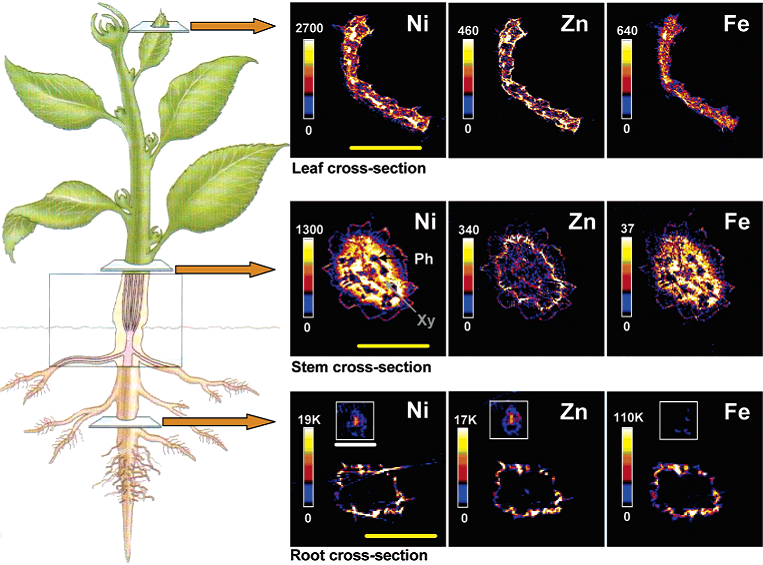
\includegraphics[width=82mm]{figs/general/xrf_tomomap}
    \end{center}
  \end{minipage} 
  & 
  \begin{minipage}{27mm}
  \vmm \vmm \vmm
  {\small{
      
      XRF Maps for Ni, Zn, and Fe in {\emph{alyssum murale}} grown in
      Ni-rich soil. 

      \vmm \vmm
      D. McNear, E. Peltier, D. Sparks, Univ of
      Delaware
      
      \vmm 
      {{\sl{Enviro Sci \& Tech}} {\bf{39}}, 2210--2218 (2005).}
    }}
  \end{minipage} \\
  \end{tabular}
\vfill
\end{slide} 
